\subsection{Аберрации в оптике}
\paragraph{Хроматическая аберрация}
Пожалуй главным недостатком оптических схем, содержащий преломляющие оптические элементы (линзы; призмы, за исключением использования их для спектроскопии) являются \imp{хроматические аберрации}. Дело в том, что показатель преломления материала линзы зависит от длины волны падающего излучения. Это приводит к тому, что положения фокуса оптической системы зависит от длины волны излучения. При наблюдениях это проявляется как радужный ореол вокруг объектов, ухудшающий качество изображения.

\begin{wrapfigure}{r}{0.5\tw}
	\centering
	\vspace{-1pc}
	\begin{tikzpicture}
		\begin{axis}[
			height	=	4.5cm,
			width	=	6cm,
			xlabel	=	{$\lambda$, мкм},
			ylabel	=	{$n(\lambda)$},
			ylabel shift	= -1 cm,
			xmin = 0.3,
			xmax = 2.5,
			ymin = 1.48,
			ymax = 1.55,
			]
			
			\addplot[smooth, domain=0.3:2.5] table[x=l, y=n] {data/crown-dispersion.txt};
		\end{axis}
	\end{tikzpicture}
	\caption{}
	\label{pic:crown-dispersion}
\end{wrapfigure}
Найдем зависимость величины хроматической аберрации от величины дисперсии материала линзы. В качестве линзы рассмотрим плосковыпуклую линзу из оптического стекла~--- \imp{крона} (BK7). Зависимость $n(\lambda)$ её показателя преломления $n$ от длины волны $\lambda$ проходящего излучения представлена на графике (см.~Рис\,\ref{pic:crown-dispersion}). Важно отметить, здесь уже нельзя считать линзу тонкой, так как само по себе понятие тонкой линзы подразумевает отсутствие разного рода аберраций и условие фокусировки лучей в одной точке (фокусе), чего не происходит на практике.

\begin{wrapfigure}[9]{r}{0.63\tw}
	\centering
	\vspace{-.8pc}
	\begin{tikzpicture}
		\footnotesize
		
		\draw [decoration={snake, segment length=.7mm, amplitude=0.2mm}, decorate] (1.35, 1) arc(-31:15:0.26);
		\draw [double, line cap=butt] (.2, 1.135) arc(180:195:0.94);
		\draw  (2.7, 0) arc(180:149:0.3);
		
		\fill [lightgray] (.5, -1.5) -- (.5, 1.5) -- (1, 1.5) arc(20:-20:4.386) -- (.5, -1.5);
		
		\draw [thick] (.5, -1.5) -- (.5, 1.5);
		\draw [thick] (1, -1.5) arc(-20:20:4.386);
		\draw [semithick, dash pattern={on 5pt off 2pt on .5pt off 2pt}] (-3.8, 0) -- (3.2, 0);
		%		\draw (-3.12, 0) node{$\times$};
		
		\draw [dashes] (-3.12, 0) -- (1.71, 1.29);
		
		\draw [semithick] (-3.8, 1.135) -- (1.12, 1.135) -- (3, 0);
		\draw [-latex] (-3.5, 1.135)-- (-1, 1.135);
		\draw [-latex] (1.12, 1.135) -- (2.25, 0.45);
		
		\draw [latex-latex] (-3.5, 0) -- (-3.5, 1.135);
		\draw [latex-latex] (1.27, -.5) -- (3, -.5);
		\draw [latex-latex] (1.12, -1.4) -- (3, -1.4);
		\draw [-latex] (0.5, -.5) -- (1.12, -.5);
		
		\draw (1.12, 1.135) -- (1.12, -1.5);
		\draw (1.27, 0) -- (1.27, -.6);
		\draw (3, 0) -- (3, -1.5);
		
		\draw (-3.5, 0.56) node[anchor=east] {$d$};
		\draw (-3.12, 0) node[anchor=north] {$C$};
		\draw (-.7, 0.6) node[anchor=north] {$R$};
		\draw (2.14, -.5) node[anchor=south] {$x$};
		\draw (2.14, -1.4) node[anchor=south] {$\frac{d}{\tg \gamma}$};
		
		\draw (.8, -1.5) node[anchor=south] {$n$};
		
		\draw (.2, 1) node[anchor=east] {$\alpha$};
		\draw (1.4, 1.07) node[anchor=west] {$\beta$};
		\draw (2.65, 0.15) node[anchor=east] {$\gamma$};
		
		\draw [fill=white] (3, 0) circle (.03);
		\draw [fill=white] (-3.12, 0) circle (.03);
	\end{tikzpicture}
	\caption{}
	\label{pic:sphere-aberrations-lens}
\end{wrapfigure}
Итак, пусть радиус кривизны выпуклой поверхности рассматриваемой плос\-ко-вы\-пук\-лой линзы равен $R$. Рассмотрим также луч, параллельный оптической оси данной линзы, на расстоянии $d$ от этой оси (см.~Рис.\,\ref{pic:sphere-aberrations-lens}). Так как передняя поверхность линзы плоская, луч, попадая в линзу, не преломляется. Преломление происходит на выходе из линзы. Нетрудно показать, что для угла падения луча на заднюю поверхность линзы $\alpha$ справедливо, что $\sin \alpha = d/R$. По закону Снеллиуса угол преломления рассматримоего луча $\beta$ определяется соотношением $\sin \beta = n \sin \alpha$. Так как угол между нормалью к выпуклой поверхности линзы и ее оптической осью равен $\alpha$, то угол $\gamma$ между преломленным лучем и оптической осью линзы равен $\beta - \alpha$.

Расстояние до точки пересечения преломлённого луча с оптической осью линзы будем отсчитывать от вершины выпуклой поверхности линзы. Расстояние $h$ между проекцией точки преломления на оптическую ось и вершиной можно найти из теоремы Пифагора:
\begin{equation*}
	h = R - \sqrt{R^2 - d^2}.
\end{equation*}
Тогда координата фокуса для лучей на расстоянии $d$ от оптической оси равно
\begin{equation}
	x = \frac{d}{\tg \gamma} - h = \frac{d}{\tg \left( \arcsin \dfrac{n d}{R} - \arcsin \dfrac{d}{R} \right)} - \left( R - \sqrt{R^2 - d^2} \right).
	\label{eq:optics-aberr-x(d)}
\end{equation}
Введём обозначение $\delta \equiv d/R$ и разделим обе части полученного равенства на $R$, чтобы перейти к относительным единицам:
\begin{equation}
	\frac{x}{R}
	= \frac{\delta}{\tg \left( \arcsin n\delta - \arcsin \delta \right)} -  1 + \sqrt{1 - \delta^2}
	~\xrightarrow{\delta \ll 1}~  \frac{1}{n - 1} - \frac{\delta^2 n^2}{2(n-1)}.\footnote{\scriptsize Вывод приближения:
	\begin{multline*}
		\frac{\delta}{\tg \left( \arcsin n\delta - \arcsin \delta \right)} -  1 + \sqrt{1 - \delta^2} =\\
		= \frac{\delta}{\tg \left[ n \delta + \dfrac{n^3 \delta^3}{6} - \delta - \dfrac{ \delta^3}{6} + o(\delta^3) \right]} -  1 + \left(1 - \frac{\delta^2}{2} + o(\delta^2) \right) =\\
		= \frac{\delta}{\tg \left[ \delta(n-1) + \dfrac{(n^3-1) \delta^3}{6} + o(\delta^3) \right]} - \frac{\delta^2}{2} + o(\delta^2) =\\
		= \frac{\delta}{\delta(n-1) + \dfrac{(n^3-1) \delta^3}{6} + \dfrac{\delta^3}{3}(n-1)^3 + o(\delta^3)} - \frac{\delta^2}{2} + o(\delta^2) =\\
		= \frac{1/(n-1)}{1 + \dfrac{\delta^2}{6}(n^2 + n + 1) + \dfrac{\delta^2}{3}(n-1)^2 + o(\delta^2)} - \frac{\delta^2}{2} + o(\delta^2) =\\
		=\frac{1}{n-1} \left[1 - \frac{\delta^2}{6} (3n^2 -3n + 3) \right] - \frac{\delta^2}{2} + o(\delta^2)
		%	= \frac{1}{n-1} - \frac{\delta^2}{2(n-1)}(n^2 - n + 1 + n - 1) + o(\delta^2)
		\simeq \frac{1}{n-1} - \frac{\delta^2 n^2}{2(n-1)}.
	\end{multline*}
	}
\end{equation}

Найдём область определения функции $x(\delta)$. Прежде всего $\delta \geqslant 0$, потому что $d$~--- это расстояние от оптической оси, которое не может быть отрицательным. С другой стороны радиус линзы не может быть больше радиуса кривизны ее поверхности, следовательно, $\delta < 1$. Однако есть ещё одно условие, которое ограничивает $\delta$ сверху. Это эффект полного внутреннего отражения. Действительно, $\sin \beta$ не может быть больше единицы, следовательно, $\sin \alpha < \sfrac{1}{n}$, а значит, $\delta < \sfrac{1}{n}$. Для стекла, коэффициент преломления которого $n \approx 1.5$, получаем, что $\delta \in [0, \sfrac{2}{3})$.

\begin{wrapfigure}{r}{0.5\tw}
	\centering
	\vspace{-1pc}
	\begin{tikzpicture}
		\begin{axis}[
			height	=	4.5cm,
			width	=	6cm,
			xlabel	=	{$\lambda$, мкм},
			ylabel	=	{$x(\lambda)$},
			ylabel shift	= -1 cm,
			xmin = 0.3,
			xmax = 2.5,
			ymin = 1.8,
			ymax = 2.1,
			]
			
			\addplot[smooth, domain=0.3:2.5] table[x=l, y=x] {data/crown-dispersion.txt};
		\end{axis}
	\end{tikzpicture}
	\caption{}
	\label{pic:crown-dispersion-x}
\end{wrapfigure}
Как будет показано далее, во избежании проявления \imp{сферической аберрации}, используют линзы с маленьким относительным отверстием ($\forall \ll 1$). Следовательно, и $\delta \ll 1$, возьмем для примера значение $\delta = 0.1$. Для него, очевидно, можно использовать приближение для $x$, поэтому при заданном значении $\delta$ выражение для $x$ принимает вид:
\begin{equation*}
	x = \frac{1}{n-1} - \frac{0.01 n^2}{2(n-1)}.
\end{equation*}
Как видно из графика данной зависимости (см.~Рис.\,\ref{pic:crown-dispersion-x}), для оптического диапазона $x(\lambda)$ принимает значения от примерно 1.85 для коротковолновой (фиолетовой) части до примерно 1.95 для красного цвета.

Чтобы компенсировать такой разбег совместно с собирающей линзой использую рассеивающую из другого материала. Объективы, где исправлена хроматическая аберрация для двух цветов и частично исправлена сферическая аберрация называют \term{ахроматами}; где хроматическая аберрация исправлена для трёх цветов, а также полностью исправлена сферическая аберрация~--- \term{апохроматами}; с более полной геометрической коррекцией~--- \term{апланатами}.

\paragraph{Сферическая аберрация}
В оптических системах, содержащих \change{сферические поверхности (линзы, зеркала)} может наблюдаться \imp{сферическая аберрация}. Суть такой аберрации состоит в том, что лучи, параллельные оптической оси, идущие на разном расстоянии от неё собираются в разных её местах. Это приводит к тому, что изображения точечных источников размываются.

\begin{wrapfigure}[12]{r}{0.55\tw}
	\centering
	\vspace{-.5pc}
	\begin{tikzpicture}
		\begin{axis}[
			height	=	5cm,
			width	=	6.5cm,
			xlabel	=	{$\delta$},
			ylabel	=	{$x(\delta)/R$},
			ylabel shift	= -1.1 cm,
			extra x ticks ={0.667},
			extra x tick labels={$\frac{1}{n}$},
			xmin=-.05,
			xmax=0.72,
			ymin=-.25,
			ymax=2.25,
			legend cell align=left,
			legend style={
			draw=none,
			fill=none,
			font=\scriptsize,
			at={(axis cs:0, 0.1)}, anchor=south west,
			row sep=.5pc,
			},
			]
			\addplot[smooth, gray] table[x=d, y=simple] {data/shere-aberrations-lens.txt};
			\addplot[smooth] table[x=d, y=x] {data/shere-aberrations-lens.txt};
			\addplot[dashes] coordinates { (0.667, -10) (0.667, 10)};
			\legend{
			$\left. \dfrac{x(\delta)}{R} \right|_{\delta \ll 1}$,
			$\dfrac{x(\delta)}{R}$,
			$\delta = \left.\dfrac{1}{n}\right|_{n=3/2}$,
			}
		\end{axis}
	\end{tikzpicture}
	\caption{}
	\label{pic:sphere-aberrations-lens-plot}
\end{wrapfigure}
Покажем наличие сферической аберрации для плосковыпуклой линзы. Рассмотрим полученное выше выражение \eqref{eq:optics-aberr-x(d)} и его приближение при $\delta \ll 1$. Зафиксируем в них $n=3/2$~--- характерное значение показателя преломления для стекла. Графики получаемых при этом зависимостей представлены на Рис.\,\ref{pic:sphere-aberrations-lens-plot}. Как видно из данных графиков, сферические аберрации проявляются уже на малых расстояниях от оптической оси.

Чтобы показать важность сферических аберраций рассмотрим небольшой телескоп рефрактор с диаметром плосковы\-пук\-ло\-во\-го\linebreak стеклянного ($n \approx 3/2$) объектива $D = 50$~мм. Характерная точность фокусировки $\Delta x$ для таких маленьких телескопов составляет около 1~мм. Установим, при каком фокусном расстоянии такого телескопа точность фокусировки нивелирует сферическую аберрацию.

При отсутствии сферической аберрации фокусное расстояние плосковыпуклового объектива $F = R/(n-1) = 2R$. Предельное значение $\delta$, которое нужно рассмотреть, соответствует лучам, проходящим через край объектива, следовательно, $\delta = D/(2R)$. Используя приближение, теперь можно записать выражение для требуемого $\Delta x$, чтобы найти необходимое для этого относительное отверситие $\forall$:
\begin{gather*}
	\Delta x = F - x(\delta) = F - x\left( \frac{D}{2R} \right),\\
	\Delta x = F - R\left( 2 - \frac{9 D^2}{4 \cdot 4R^2} \right),\\
	\Delta x = \frac{9D^2}{16R} = \frac{9D^2}{16F} = \frac{9}{16} D \forall;\\
	\therefore \forall = \frac{\Delta x \cdot 16}{9D} = 0.036.
\end{gather*}

\begin{wrapfigure}[9]{r}{0.5\tw}
	\centering
	\vspace{-.8pc}
	\begin{tikzpicture}
		\footnotesize
		
		\draw [decoration={snake, segment length=.7mm, amplitude=0.2mm}, decorate] (1.35, 1) arc(-31:15:0.26);
		\draw (.2, 1.135) arc(180:209:0.94);
		\draw (-2.18, 0) arc(0:15:0.94);
		
		\fill [lightgray] (1.5, -1.5) -- (1.5, 1.5) -- (1, 1.5) arc(20:-20:4.386) -- (1.5, -1.5);
		
		\draw [thick] (1, -1.5) arc(-20:20:4.386);
		\draw [semithick, dash pattern={on 5pt off 2pt on .5pt off 2pt}] (-3.8, 0) -- (1.7, 0);
		
		\draw [dashes] (-3.12, 0) -- (1.71, 1.29);
		
		\draw [semithick] (-3.8, 1.135) -- (1.12, 1.135) -- (-.85, 0);
		\draw [-latex] (-3.5, 1.135)-- (-1, 1.135);
		\draw [-latex] (1.12, 1.135) -- (-.06, 0.45);
		
		\draw [latex-latex] (-3.5, 0) -- (-3.5, 1.135);
		\draw [latex-latex] (-.85, -1.3) -- (1.27, -1.3);
		
		\draw (1.27, 0) -- (1.27, -1.5);
		\draw (-.85, 0) -- (-.85, -1.5);
		
		\draw (-3.5, 0.56) node[anchor=east] {$d$};
		\draw (-0.85, 0) node[anchor=north east] {$F$};
		\draw (-3.12, 0) node[anchor=south] {$C$};
		\draw (-1.2, 0.5) node[anchor=south] {$R$};
		\draw (0.27, -1.3) node[anchor=south] {$x_F(d)$};
		
		\draw (.2, 1) node[anchor=east] {$\alpha$};
		\draw (-2.2, .15) node[anchor=west] {$\alpha$};
		\draw (.3, .7) node[anchor=east] {$\alpha$};
		
		\draw [fill=white] (-0.85, 0) circle (.03);
		\draw [fill=white] (-3.12, 0) circle (.03);
	\end{tikzpicture}
	\caption{}
	\label{pic:sphere-aberrations-mirrow}
\end{wrapfigure}
Найдем теперь величину аберрации сферического зеркала.\linebreak Пусть $R$~--- радиус кривизны зеркал. Рассмотрим луч, идущий параллельно оптической оси зеркала на расстоянии $d$ от неё. Он падает на зеркало под углом $\alpha$, причем $\sin \alpha = d/R$. В силу закона отражения: угол падения равен углу отражения, то есть угол отражения также равен $\alpha$. Кроме того, угол между нормалью к зеркалу в точке отражения и оптической осью зеркала также равен $\alpha$ как вертикальный. Следовательно треугольник {\slshape центр кривизны зеркала ($C$) -- точка отражения ($A$) -- точка пересечения отраженного луча с оптической осью (F)} является равнобедренным. Значит расстояние $x_F(d)$ от центра зеркала до <<фокуса>> $F$ можно найти как
\begin{gather*}
	x_F(d) = R - \frac{R}{2} \cdot \frac{1}{\cos\alpha} = R - \frac{R}{2\sqrt{1 - \sin^2 \alpha}}  = R  - \frac{R}{2\sqrt{1 - \dfrac{d^2}{R^2}}};\\
	\left. \frac{x_F(d)}{R} \right|_{d \ll R} \simeq  1  - \frac{1}{2\left(1 - \dfrac{d^2}{2R^2} \right)} \simeq  1 - \frac{1}{2}\left(1 + \dfrac{d^2}{2R^2} \right)  = \frac{1}{2} -  \dfrac{d^2}{4R^2}.
\end{gather*}
\begin{wrapfigure}[12]{r}{0.55\tw}
	\centering
	\vspace{-.5pc}
	\begin{tikzpicture}
		\begin{axis}[
			height	=	5cm,
			width	=	6.5cm,
			xlabel	=	{$d/R$},
			ylabel	=	{$x(d)/R$},
			ylabel shift	= -1.1 cm,
			extra x ticks ={sqrt(2)/2},
			extra x tick labels={$\frac{\sqrt{2}}{2}$},
			xmin=-.05,
			xmax=0.85,
			ymin=.15,
			ymax=0.55,
			legend cell align=left,
			legend style={
			draw=none,
			fill=none,
			font=\scriptsize,
			at={(axis cs:0, .2)}, anchor=south west,
			row sep=.5pc,
			},
			]
			\addplot[smooth, gray] table[x=d, y=simple] {data/sphere-aberrations-mirrow.txt};
			\addplot[smooth] table[x=d, y=x] {data/sphere-aberrations-mirrow.txt};
			\addplot[dashes] coordinates { (sqrt(2)/2, -10) (sqrt(2)/2, 10)};
			\legend{
			$\left. \dfrac{x_F(d)}{R} \right|_{d \ll R}$,
			$\dfrac{x_F(d)}{R}$,
			$ \dfrac{d}{R} = \dfrac{\sqrt{2}}{2}$,
			}
		\end{axis}
	\end{tikzpicture}
	\caption{}
\end{wrapfigure}
Отсюда получается, что фокус сферического зеркала находится ровно между центром кривизны зеркала и центром этого зеркала. Однако в силу сферической аберрации возникает ошибка фокусировки порядка $d/R$, которая размывает изображение. Причём при $d > R\sqrt{2}/2$ лучи не <<разворачиваются>>, следовательно, не вносят вклада в изображение, так как приходят на приемник с другой стороны.

Для компенсации сферической аберрации используют различные линзы-корректоры, однако они помогают лишь частично избавиться от неё. \change{Поэтому в современных рефлекторах используются параболические зеркала, не подверженные сферическим аберрациям.}

%Напоследок нужно отметить, что сферические аберрации

\paragraph{Астигматизм} Ещё один вид аберраций оптических систем состоящий в разности радиусов кривизны оптических элементов в двух перпендикулярных направлениях. Такое возможно, например, в случае большой массы линзы или зеркала. Когда данный оптический элемент долгое время находится в вертикальном положении (оптическая ось горизонтальна), он деформируется: вдоль горизонтали радиус кривизны сохраняется, а по вертикали из-за сжатия уменьшается.

\imp{Астигматизм} проявляется в том, что пучок лучей, исходящих из какой-либо точки, после прохождения через оптическую систему собирается не в одной точке, а на двух взаимно перпендикулярных отрезках, расположенных на некотором расстоянии друг от друга. Изображения промежуточных сечений имеют форму эллипсов.

\paragraph{Кома}

\begin{wrapfigure}[13]{l}{0.4\tw}
	\centering
	\vspace{-1pc}
	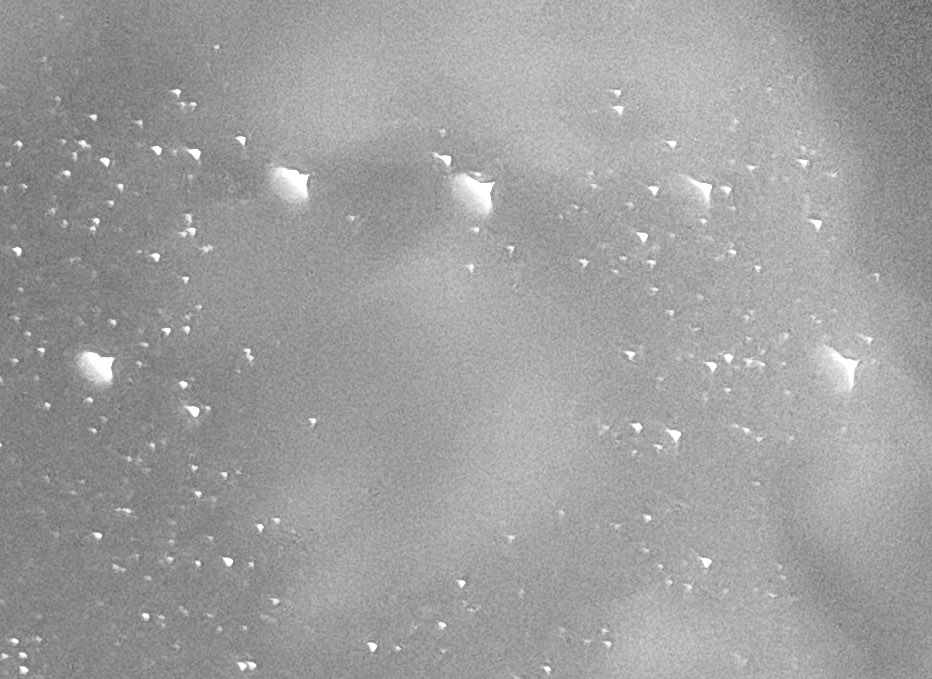
\includegraphics[width=0.4\tw]{img/optics-aberrations-coma.jpg}
	\caption{Изображение <<хвоста>> Большой Медведицы, полученное с помощью широкоугольного объектива, страдающего ярко выраженной комой.}
	\label{pic:optics-aberrations-coma}
\end{wrapfigure}
Один из видов аберраций оптических систем~--- аберрация широкого пучка световых лучей, проходящий наклонно к оптической оси системы, как и \imp{сферическая аберрация}, обусловлена неодинаковым преломлением световых лучей различными участками линзовых компонент системы. Кома приводит к нарушению центрированности светового пучка. В результате такой аберрации изображение точки имеет вид несимметричного пятна (см.~Рис.\,\ref{pic:optics-aberrations-coma}), по форме напоминающего запятую (англ. {\itshape comma}).

\begin{figure}[h]
	\centering
	\begin{tikzpicture}[ipe stylesheet, scale=1.1]
		%  \useasboundingbox (200, 500) rectangle (550, 750);
		\fill [lightgray] (336, 704) -- (336, 576) -- (384, 576) arc[start angle=-26.5651, end angle=26.5651, radius=143.1084] -- (336, 704);
		\draw[ipe pen fat]
		(384, 576)
		arc[start angle=-26.5651, end angle=26.5651, radius=143.1084];
		\draw[ipe pen fat]
		(336, 704)
		-- (336, 576);
		
		\draw[ipe pen heavier, ipe dash dash dotted]
		(224, 640)
		-- (500, 640);
		\draw[ipe dash dashed]
		(224, 688)
		-- (380, 688);
		\draw[ipe dash dashed]
		(304, 592)
		-- (368, 592);
		\draw[ipe dash dashed]
		(256, 640)
		-- (410.7052, 705.7731);
		\draw[ipe dash dashed]
		(256, 640)
		-- (415.3607, 594.5412);
		\draw[ipe pen heavier]
		(252, 664)
		-- (336, 688)
		-- (388, 696)
		-- (464, 650)
		-- (393, 601)
		-- (336, 592)
		-- (280, 576);
		\filldraw[fill=white]
		(435, 640) [double, line cap = butt]
		arc[start angle=180, end angle=215, radius=15];
		\node[ipe node]
		at (251.993, 630.085) {$C$};
		\draw
		(356, 700)
		-- (256, 640)
		-- (356, 580);
		\draw
		(350, 690)
		arc[start angle=9.2524, end angle=42, radius=9.7017];
		\draw
		(380, 688) [decoration={zigzag, segment length=1.1mm, amplitude=0.3mm}, decorate]
		arc[start angle=0, end angle=8.9, radius=45];
		\draw
		(316, 687.9682)
		arc[start angle=-180, end angle=-164.0101, radius=20];
		\draw
		(350, 690) [decoration={snake, segment length=1mm, amplitude=0.3mm}, decorate]
		arc[start angle=-171.1895, end angle=-157.2715, radius=38];
		\draw
		(397.3793, 690)
		arc[start angle=-20, end angle=20, radius=15];
		\draw
		(272.7114, 640.2703) [double,  line cap=butt]
		arc[start angle=0.9936, end angle=23.3266, radius=16.5778];
		\draw
		(280.6909, 632.9696)
		arc[start angle=-15.3798, end angle=0.7105, radius=25.6239];
		\node[ipe node]
		at (364.414, 642.015) {$h$};
		\node[ipe node]
		at (326.338, 662.276) {$R$};
		\node[ipe node]
		at (326.556, 621.048) {$R$};
		\draw[{ipe fptarc[ipe arrow small]}-{ipe fptarc[ipe arrow small]}]
		(240, 688)
		-- (240, 640);
		\node[ipe node]
		at (233.078, 660.549) {$d$};
		\node[ipe node]
		at (364.414, 642.015) {$h$};
		\node[ipe node]
		at (294.96, 666.059) {$l$};
		\node[ipe node]
		at (276.734, 643.661) {$\eta_1$};
		\node[ipe node]
		at (284.917, 634.094) {$\eta_2$};
		\node[ipe node]
		at (307, 683.074) {$\alpha$};
		\node[ipe node]
		at (383, 688) {\small $\beta$};
		\node[ipe node]
		at (342, 683) {\small $\gamma_1$};
		\node[ipe node]
		at (402, 693) {$\delta_1$};
		\draw
		(464, 650)
		-- (500, 620);
		\node[ipe node]
		at (425, 633) {$\omega_2$};
		\node[ipe node]
		at (457, 656) {$(x, y)$};
		\node[ipe node]
		at (408, 602) {$\delta_2$};
		\node[ipe node]
		at (366.698, 589.106) {$\beta$};
		\node[ipe node]
		at (363.462, 601.476) {$\gamma_2$};
		\node[ipe node]
		at (306.222, 586.462) {$\alpha$};
		\draw
		(316, 591.9788)
		arc[start angle=180, end angle=194.6129, radius=20];
		\draw
		(327.0296, 597.2938)
		arc[start angle=148.7026, end angle=178.4025, radius=10.533];
		\node[ipe node]
		at (314.996, 595.309) {$\xi$};
		\node[ipe node]
		at (355, 695) {\small $\xi - \beta$};
		\node[ipe node]
		at (325, 692.319) {$A_1$};
		\node[ipe node]
		at (388, 703) {$B_1$};
		\node[ipe node]
		at (324, 582) {$A_2$};
		\node[ipe node]
		at (393, 591) {$B_2$};
		\node[ipe node]
		at (338, 643) {$O$};
		\draw
		(362.1296, 591.989)
		arc[start angle=0.3563, end angle=9.2262, radius=26.1304];
		\draw
		(374.9012, 606.1184)
		arc[start angle=163.6381, end angle=187.6335, radius=19.4597];
		\draw
		(404.9644, 597.6586)
		arc[start angle=-15.516, end angle=38, radius=11.8867];
		%  \draw
		%    (580.705, 634.3486)
		%     arc[start angle=-17.9201, end angle=0.7153, radius=17.6622];
		%  \node[ipe node]
		%     at (583.258, 634.438) {$\omega_1$};
		
		%    		\foreach \x in {200, 210,...,500} {
		%				\draw [line width=.1pt] (\x, 500) -- (\x, 800);
		%				};
		%
		%				\foreach \x in {200, 300,...,500} {
		%				\draw [line width=.4pt] (\x , 500) -- (\x, 800);
		%				};
		%
		%				\foreach \y in {500, 510,...,800} {
		%				\draw [line width=.1pt] (200, \y) -- (500, \y);
		%				};
		%
		%				\foreach \y in {500, 600,...,800} {
		%				\draw [line width=.4pt] (200, \y) -- (500, \y);
		%				};
		
		\pic[ipe mark small, fill=white]
		at (256, 640) {ipe fdisk};
		\pic[ipe mark small, fill=white]
		at (336, 688) {ipe fdisk};
		\pic[ipe mark small, fill=white]
		at (388, 696) {ipe fdisk};
		\pic[ipe mark small, fill=white]
		at (336, 592) {ipe fdisk};
		\pic[ipe mark small, fill=white]
		at (464, 650) {ipe fdisk};
		\pic[ipe mark small, fill=white]
		at (393.5264, 600.6558) {ipe fdisk};
		\pic[ipe mark small, fill=white]
		at (336, 640) {ipe fdisk};
		
	\end{tikzpicture}
	\caption{}
	\label{pic:optics-aberrations-coma1}
\end{figure}

Найдем положение фокуса светового пучка, идущего под углом $\alpha$ к оптической оси. Для этого рассмотрим два луча из него, вместе с оптической осью лежащих в одной плоскости, таких, что точки преломления их передней (плоской) поверхностью линзы $A_1$ и $A_2$ лежат на расстоянии $d$ от оптической оси линзы (см.~Рис.\,\ref{pic:optics-aberrations-coma1}).

Пусть толщина линзы~--- расстояние вдоль оптической оси от вершины выпуклой поверхности, до центра плоской поверхности $O$, равно $h$. А радиус кривизны выпуклой поверхности равен $R$. Тогда расстояние $l$ от центра кривизны задней (выпуклой) поверхности линзы до точек $A_1$ и $A_2$ можно найти из теоремы Пифагора для треугольника $\triangle COA_{1,2}$:
\begin{equation*}
	l = \sqrt{(R - h)^2 - d^2}.
\end{equation*}
Равные углы $\angle A_{1,2} C O$ обозначим за $\xi$, где
\begin{equation*}
	\xi = \arcsin \frac{d}{l}.
\end{equation*}

Угол падения рассматриваемых лучей на плоскую поверхность линзы равен $\alpha$, следовательно, по закону Снеллиуса угол преломления $\beta$ определяется выражением
\begin{equation*}
	\beta = \arcsin \frac{\sin \alpha}{n},
\end{equation*}
где $n$~--- показатель преломления линзы. Обозначим углы падения верхнего и нижнего луча на заднюю поверхность линзы $\gamma_{1,2}$ соответственно. А точки преломления лучей задней поверхностью соответственно $B_{1,2}$. Запишем теорему синусов для треугольников $\triangle C A_{1,2} B_{1,2}$, чтобы найти углы $\gamma_{1,2}$ соответственно:
\begin{gather*}
	\frac{R}{\sin (180^\circ - (\xi \mp \beta))} = \frac{l}{\sin \gamma_{1,2}},\\
	\therefore \gamma_1 = \arcsin \frac{l\sin (\xi \mp \beta)}{R}.
\end{gather*}

Чтобы найти координаты точек $B_{1,2}$, определим сначала углы $ \eta_{1,2} \equiv \angle B_{1,2} C O$:
\begin{equation*}
	\eta_{1,2} = \xi - \Big[180^\circ - \gamma_{1,2} - \big(180^\circ - \left(\xi \mp \beta\right)\big)\Big] = \gamma_{1,2} \pm \beta.
\end{equation*}

Введем теперь декартову систему координат, за начало отсчета примем центр кривизны выпуклой поверхности линзы, ось $x$ направим вдоль оптической оси вправо, ось $y$ перпендикулярно вверх. В такой системе координаты точки $B_{1,2}$ задаются векторами
\begin{equation*}
	\begin{pmatrix}
		x_{1,2}\\
		y_{1,2}
	\end{pmatrix}
	= R
	\begin{pmatrix}
		\cos \eta_{1,2}\\
		\sin \eta_{1,2}
	\end{pmatrix}.
\end{equation*}
Остается воспользоваться законом Снеллиуса для определения углов $\delta_{1,2}$:
\begin{equation*}
	\delta_{1,2} = \arcsin \left( n \sin \gamma_{1,2} \right).
\end{equation*}

Поиск координат  $(x,y)$ точки пересечения лучей, вышедших из линзы начнём с поиска абсциссы. Можно заметить, что она должно удовлетворять уравнению
\begin{gather*}
	-(x - x_1) \tg \omega_1 + (x - x_2) \tg \omega_2 = y_1 + y_2,\\
	\therefore x = \frac{y_1 + y_2 - x_1\tg \omega_1 + x_2 \tg \omega_2}{\tg \omega_2 - \tg \omega_1};
\end{gather*}
где $\omega_1 = \eta_1 - \delta_1$, а $\omega_2 = -\eta_2 + \delta_2$. Теперь не сложно найти координату $y$ <<фокуса>>:
\begin{equation*}
	y = y_1 + (x - x_1) \tg \omega_1 = y_2 + (x - x_2) \tg \omega_2.
\end{equation*}

Продемонстрируем полученные зависимости (см.~Рис.\,\ref{pic:coma}), при следующих параметрах: $R = 1$, $h = 0.3$, $\alpha = 50^\circ$, $n=1.5$.

\begin{figure}
	\begin{subfigure}{0.49\tw}
		\begin{tikzpicture}
			\begin{axis}[
				height	=	5cm,
				width	=	6cm,
				xlabel	=	{$d$},
				ylabel	=	{},
				ylabel shift	= -1.1 cm,
				%			extra x ticks ={sqrt(2)/2},
				%			extra x tick labels={$\frac{\sqrt{2}}{2}$},
				xmin=0,
				xmax=0.5,
				ymin=.6,
				ymax=2,
				legend cell align=left,
				legend style={
				draw=none,
				fill=none,
				font=\scriptsize,
				at={(axis cs:.5, 2)}, anchor=north east,
%				row sep=.5pc,
				},
				]
				\addplot[smooth, gray] table[x=d, y=x] {data/coma.txt};
				\addplot[smooth] table[x=d, y=y] {data/coma.txt};
				\addplot[dashes] coordinates { (0.359606, -10) (0.359606, 1.6)};
				\legend{
				$x(d)$,
				$y(d)$,
%				$d:~\gamma_2(d)=\arcsin\frac{1}{n}$ 
				}
			\end{axis}
		\end{tikzpicture}
%		\caption{}
	\end{subfigure}
	\hfill
	\begin{subfigure}{0.49\tw}
		\begin{tikzpicture}
			\begin{axis}[
				height	=	5cm,
				width	=	6cm,
				xlabel	=	{$x$},
				ylabel	=	{$y$},
				ylabel shift	= -1.1 cm,
				%			extra x ticks ={sqrt(2)/2},
				%			extra x tick labels={$\frac{\sqrt{2}}{2}$},
				xmin=1.2,
				xmax=2,
				ymin=.6,
				ymax=1.1,
				]
				\addplot[only marks, mark = o, mark options={scale=0.2, black}] table[x=x, y=y] {data/coma.txt};
			\end{axis}
		\end{tikzpicture}
%		\caption{}
	\end{subfigure}
	\caption{}
	\label{pic:coma}
\end{figure}

